\documentclass[11pt,a4paper]{article}
\usepackage{fontspec}
\setmainfont{TeX Gyre Pagella}
\newfontfamily\headfont{Inter}[UprightFont=*-ExtraBold,BoldFont=*-ExtraBold,Extension=.otf,Path=/usr/share/fonts/opentype/inter/]
\newfontfamily\cjk{Noto Serif CJK SC}
\usepackage[a4paper,margin=2.3cm]{geometry}
\usepackage{graphicx,booktabs,float,caption,array,xcolor,longtable}
\usepackage{xurl}
\usepackage[hidelinks]{hyperref}
\usepackage{titlesec}
\usepackage[round]{natbib}
\usepackage{setspace}
\setstretch{1.05}
\renewcommand{\topfraction}{0.9}
\renewcommand{\bottomfraction}{0.8}
\renewcommand{\textfraction}{0.1}
\renewcommand{\floatpagefraction}{0.75}
\setlength{\parindent}{0pt}
\setlength{\parskip}{0.55em}
\titleformat{\section}{\headfont\Large}{\thesection}{0.8em}{}
\titleformat{\subsection}{\headfont\large}{\thesubsection}{0.8em}{}
\captionsetup{font=small,labelfont=bf}
\urlstyle{same}
\hypersetup{pdftitle={The Colours of the World's Place Names},pdfauthor={Tristan Hotham}}

\begin{document}
\begin{center}
{\Large\bfseries The Colours of the World's Place Names\par}
\vspace{0.4em}
{\large Black, white, red, green, blue and yellow in 138,453 names from GeoNames,\\in 20 languages\par}
\vspace{1.2em}
{\large Tristan Hotham\par}
\vspace{0.3em}
{\small Independent researcher\\
ORCID: 0000-0003-4931-9349\\
DOI: https://doi.org/10.5281/zenodo.24043682\par}
\vspace{0.8em}
2026
\end{center}

\begin{quote}
\small
\begin{center}\textbf{Abstract}\end{center}
Places all over the world are named after their colour: Black Creek, Río Blanco, Cerro Colorado, Kara Su, Krasnaya Gorka, Baishui. I extract colour names from GeoNames, the largest open gazetteer, with a classifier written separately for each of 20 languages or language groups, and check it on review samples of up to 50 names for each colour and language (4,370 names; 99\% judged correct after tuning) and of 50 names for each rule of a second, wider pass (299 of 300 correct). The main set holds 138,453 natural features and settlements in 214 countries and territories. White is the commonest colour (26.5\%), then black (23.2\%) and red (20.6\%); without the very numerous Chinese and Japanese names black edges ahead (27.3\% against 25.7\%) and blue is rare everywhere (5.5\% overall). The colour depends on the kind of place: weighting languages equally, rivers are the blackest kind (37.2\% black, blacker than their language's average in 14 of 17 languages) and springs the whitest (42.7\%), while mountains are only weakly white. Each language has a favourite: svart in the Nordic languages, siāh in Persian, kara and ak in the Turkic languages, blanco and colorado in Spanish, bai and huang in Chinese. In the 102 countries with at least 30 names, the commonest colour is white in 35, black in 35 and red in 21. Red is partly political: 21.9\% of East Slavic and 29.8\% of Chinese red names are revolutionary. Names of earth, soil and clay are no redder than names in general.

\textbf{Keywords:} toponymy; colour terms; place names; GeoNames; basic colour terms; historical geography; maps
\end{quote}

\section{Introduction}
Colour is one of the oldest ways of naming a place. A peat-dark stream, a chalk spring, a hill of red soil or a green island is named for what it looks like, and these names are among the most transparent in any language. The words for colour are also among the most studied words in linguistics: since \citet{berlinkay} it has been argued that languages gain their basic colour terms in a broadly fixed order, black and white (or dark and light) first, then red, then green and yellow, then blue.

This study asks how colours are used in the names of places across the world. Which colours are used most, and does that follow the order of colour terms? Do kinds of place have characteristic colours, black rivers or white mountains? Which colours does each language favour, and which country's names are blackest or whitest? And how much of the red in place names is the colour of the ground? It accompanies an interactive map of every name (\url{https://maps.tristanhotham.com/colour-names/}).

\section{Data}
\textbf{GeoNames.} GeoNames \citep{geonames} is an open gazetteer of about 13 million features, each with a name, an ASCII form, alternate names in other languages and scripts, coordinates, a feature class and code (stream, mountain, populated place and so on) and a country code. It is released under CC BY 4.0. It is built from national gazetteers and its density varies greatly: the United States, Mexico, China, Norway and Iran are covered in great detail, much of Africa and South Asia thinly.

\textbf{The candidates.} Two searches on colour words were run over the full allCountries dump and kept 252,615 rows. The first (185,388 rows) took whole words in English and the Romance languages; the start of words in German, Dutch, the Nordic languages, Polish and Russian; whole words in the Turkic, Arabic and Persian romanisations; and the colour characters in the Chinese and Japanese alternate names. A second, wider pass (67,227 rows) added compounds and languages the first had missed: English compounds in Britain, Ireland and the former colonies (Blackburn, Whitby, Greenwich, Redcar), Turkic compounds (Aksu, Karakol, Kızılırmak, Göksu), Norwegian and Danish \textit{kvit} and \textit{hvid}, Mongolian (\textit{khar}, \textit{tsagaan}, \textit{ulaan}, \textit{nogoon}, \textit{khökh}, \textit{shar}), Hindi, Urdu and Nepali (\textit{kala}, \textit{safed}, \textit{lal}, \textit{hara}, \textit{nila}, \textit{pila}) and Korean. These are candidates, most of which are not colour names in the sense meant here.

\textbf{Other sources.} Country outlines are from Natural Earth \citep{naturalearth}; the interactive map uses the Inked World map style \citep{inkmap} on OpenStreetMap data served by OpenFreeMap.

\section{Methods}
\subsection{A classifier for each language}
A colour word in a place name is often something else: a surname (White's Creek, Colonia Rojas, Huangjiacun), a saint (Santa Blanca), a person (Red Nichols Lake), a state (Colorado Springs), a plant or animal (Red Oak, Blue Jay), a revolutionary slogan (Krasnyy Oktyabr'), or a different word that looks the same (Rotterdam, Belgorod's neighbour Belovo, Finnish \textit{vita-}). The classifier therefore has a rule set for each language (Table~\ref{tab:rules}). A name passes when one of its words is a colour word of a language spoken in the country where the place lies, in a form that language uses for the colour: the plain or inflected adjective, or the first part of a compound whose second part is a landscape word from a list (German \textit{Schwarz-wald}, Norwegian \textit{Svart-berget}, Afrikaans \textit{Wit-rivier}, Turkish \textit{Kızıl-ırmak}, Russian \textit{Krasno-yarsk}). Each language has a stop-list: names after a saint, a possessive (\textit{X's}), family-name endings (Polish \textit{-ów}, \textit{-owo}; Russian \textit{-ov}, \textit{-ovo}); in the United States, Canada and Australia, Spanish \textit{negro} and \textit{colorado} count only with a Spanish word beside them, since Negro Creek is named for people and Colorado City for the state. Chinese and Japanese names are read only in their own characters, from the alternate names, since romanised syllables such as \textit{bai} or \textit{hong} have many other meanings; Chinese names whose colour character is followed by a word for family or house (\textit{jia}, \textit{zhuang}) are treated as family names, and pasture names written in sound for Tibetan and Mongolian words are dropped. The rules of the second pass are stricter still (Table~\ref{tab:supp}). An English compound must end in a landscape element of English place names (\textit{-burn}, \textit{-pool}, \textit{-by}, \textit{-church}, \textit{-wich}, \textit{-water}); \textit{Red-} takes a short list (\textit{-hill}, \textit{-car}, \textit{-cliff}), since it is often Old English \textit{hr\=eod}, reed, or Cornish \textit{rhyd}, ford (Redruth, Redbourn, Redmire), and bare \textit{Whit-} counts only in Britain and Ireland (Whitby, Whitchurch), since Whitney and Whittington come from the personal name Hwita; in North America, Australia, New Zealand and South Africa common surnames (Blackburn, Greenwood, Whitley) and towns named after people (Greenville) are stopped. A Turkic stem must start the word and be followed by a landscape word (\textit{Ak-su}, \textit{Kara-kol}, \textit{Kızıl-ırmak}), with stops for \textit{karaca} (roe deer), \textit{akar} (flowing) and the like. Mongolian words count as whole words or hyphenated compounds, never Russian \textit{shar}, a strait. Hindi and Urdu words count only beside a landscape word (Kala Pani, Lal Tibba), which keeps out personal names (Lal Khan, Moti Lal) and the goddess Kali but also most red and white names. Korean names count only where GeoNames gives the colour hanja ({\cjk 紅} for hong, as hong is also the family name {\cjk 洪}) or where a hangul compound is unambiguous ({\cjk 흑}, black; {\cjk 백석}, white stone; {\cjk 청룡}, blue dragon; {\cjk 황토}, yellow earth). The single East Asian character {\cjk 青} (qing in Chinese, ao in Japanese), which covers blue and green, is kept as its own category, blue-green.

Two flags are kept rather than dropped. English names in which the colour belongs to a plant or animal (Red Oak, White Pine, Blackbird) are flagged and left out of the main set (2,900 names). Red names from the Soviet and Chinese revolutionary vocabulary (with \textit{Oktyabr'}, \textit{Zvezda}, \textit{Partizan}, {\cjk 红旗} Red Flag, {\cjk 红星} Red Star and the like) are flagged as political and kept, since they are red names, but reported apart.

\begin{table}[tbp]\centering\footnotesize\caption{The second pass: candidate rows found by each search, names accepted into the main set, and review sample judged correct.}\label{tab:supp}\begin{tabular}{lrrr}\toprule Rule & Candidates & Accepted & Correct\\\midrule
Turkic compounds & 32,503 & 9,395 & 50 of 50\\
English compounds & 24,626 & 2,254 & 49 of 50\\
Norwegian kvit, Danish hvid & 1,854 & 1,374 & 50 of 50\\
Mongolian & 2,809 & 793 & 50 of 50\\
Hindi, Urdu and Nepali & 2,546 & 238 & 50 of 50\\
Korean & 2,889 & 184 & 50 of 50\\
\bottomrule\end{tabular}\end{table}

\subsection{Kinds of place and the main set}
GeoNames feature codes are grouped into nine kinds of place: rivers, streams and wadis; lakes, ponds and marshes; springs and wells; seas, bays and coasts; mountains and hills; rocks, cliffs and islands; valleys, gorges and passes; plains, deserts, woods and other land; and towns and villages. Buildings, farms, mines, hotels, parks, roads, administrative areas and undersea features (35,478 accepted names) are left out of the main set, because they often take a colour from an owner, a brand or another place.

\subsection{Review}
For every language and colour I read a sample of up to 50 accepted names, drawn in a fixed pseudo-random order (an MD5 hash of the GeoNames identifier), and judged whether the word is the colour there. The samples were used to tune the rules, and the final precision is measured on the samples drawn after tuning, so it is optimistic: names the tuning removed were found in these samples. In all I read 4,459 different names.

\subsection{Comparisons}
Shares of each colour are given for all names pooled, and, where noted, with each language weighted equally (languages with at least 30 names of the kind of place in question), so that the 29,530 Chinese names, most of them villages, do not dominate. Countries are compared on the most common colour among their names and on the ratio of black to white names, with half a name added to each count. Names of earth, soil, sand and clay are found by words in the name (\textit{tierra}, \textit{terra}, \textit{barro}, \textit{glina}, \textit{khāk}, \textit{kum} and others, and the characters {\cjk 土} and {\cjk 泥}).

\section{Results}
\subsection{The whole map}
The main set holds 138,453 names in 214 countries and territories (Figure~\ref{fig:world}): 77,115 natural features and 61,338 settlements. The density of dots follows the density of the gazetteer: the United States, Mexico, China, Norway, Russia, Kazakhstan, Turkey and Iran stand out. The second pass contributes 14,238 names, 9,395 of them Turkic compounds and 2,254 English ones.

\begin{figure}[tbp]\centering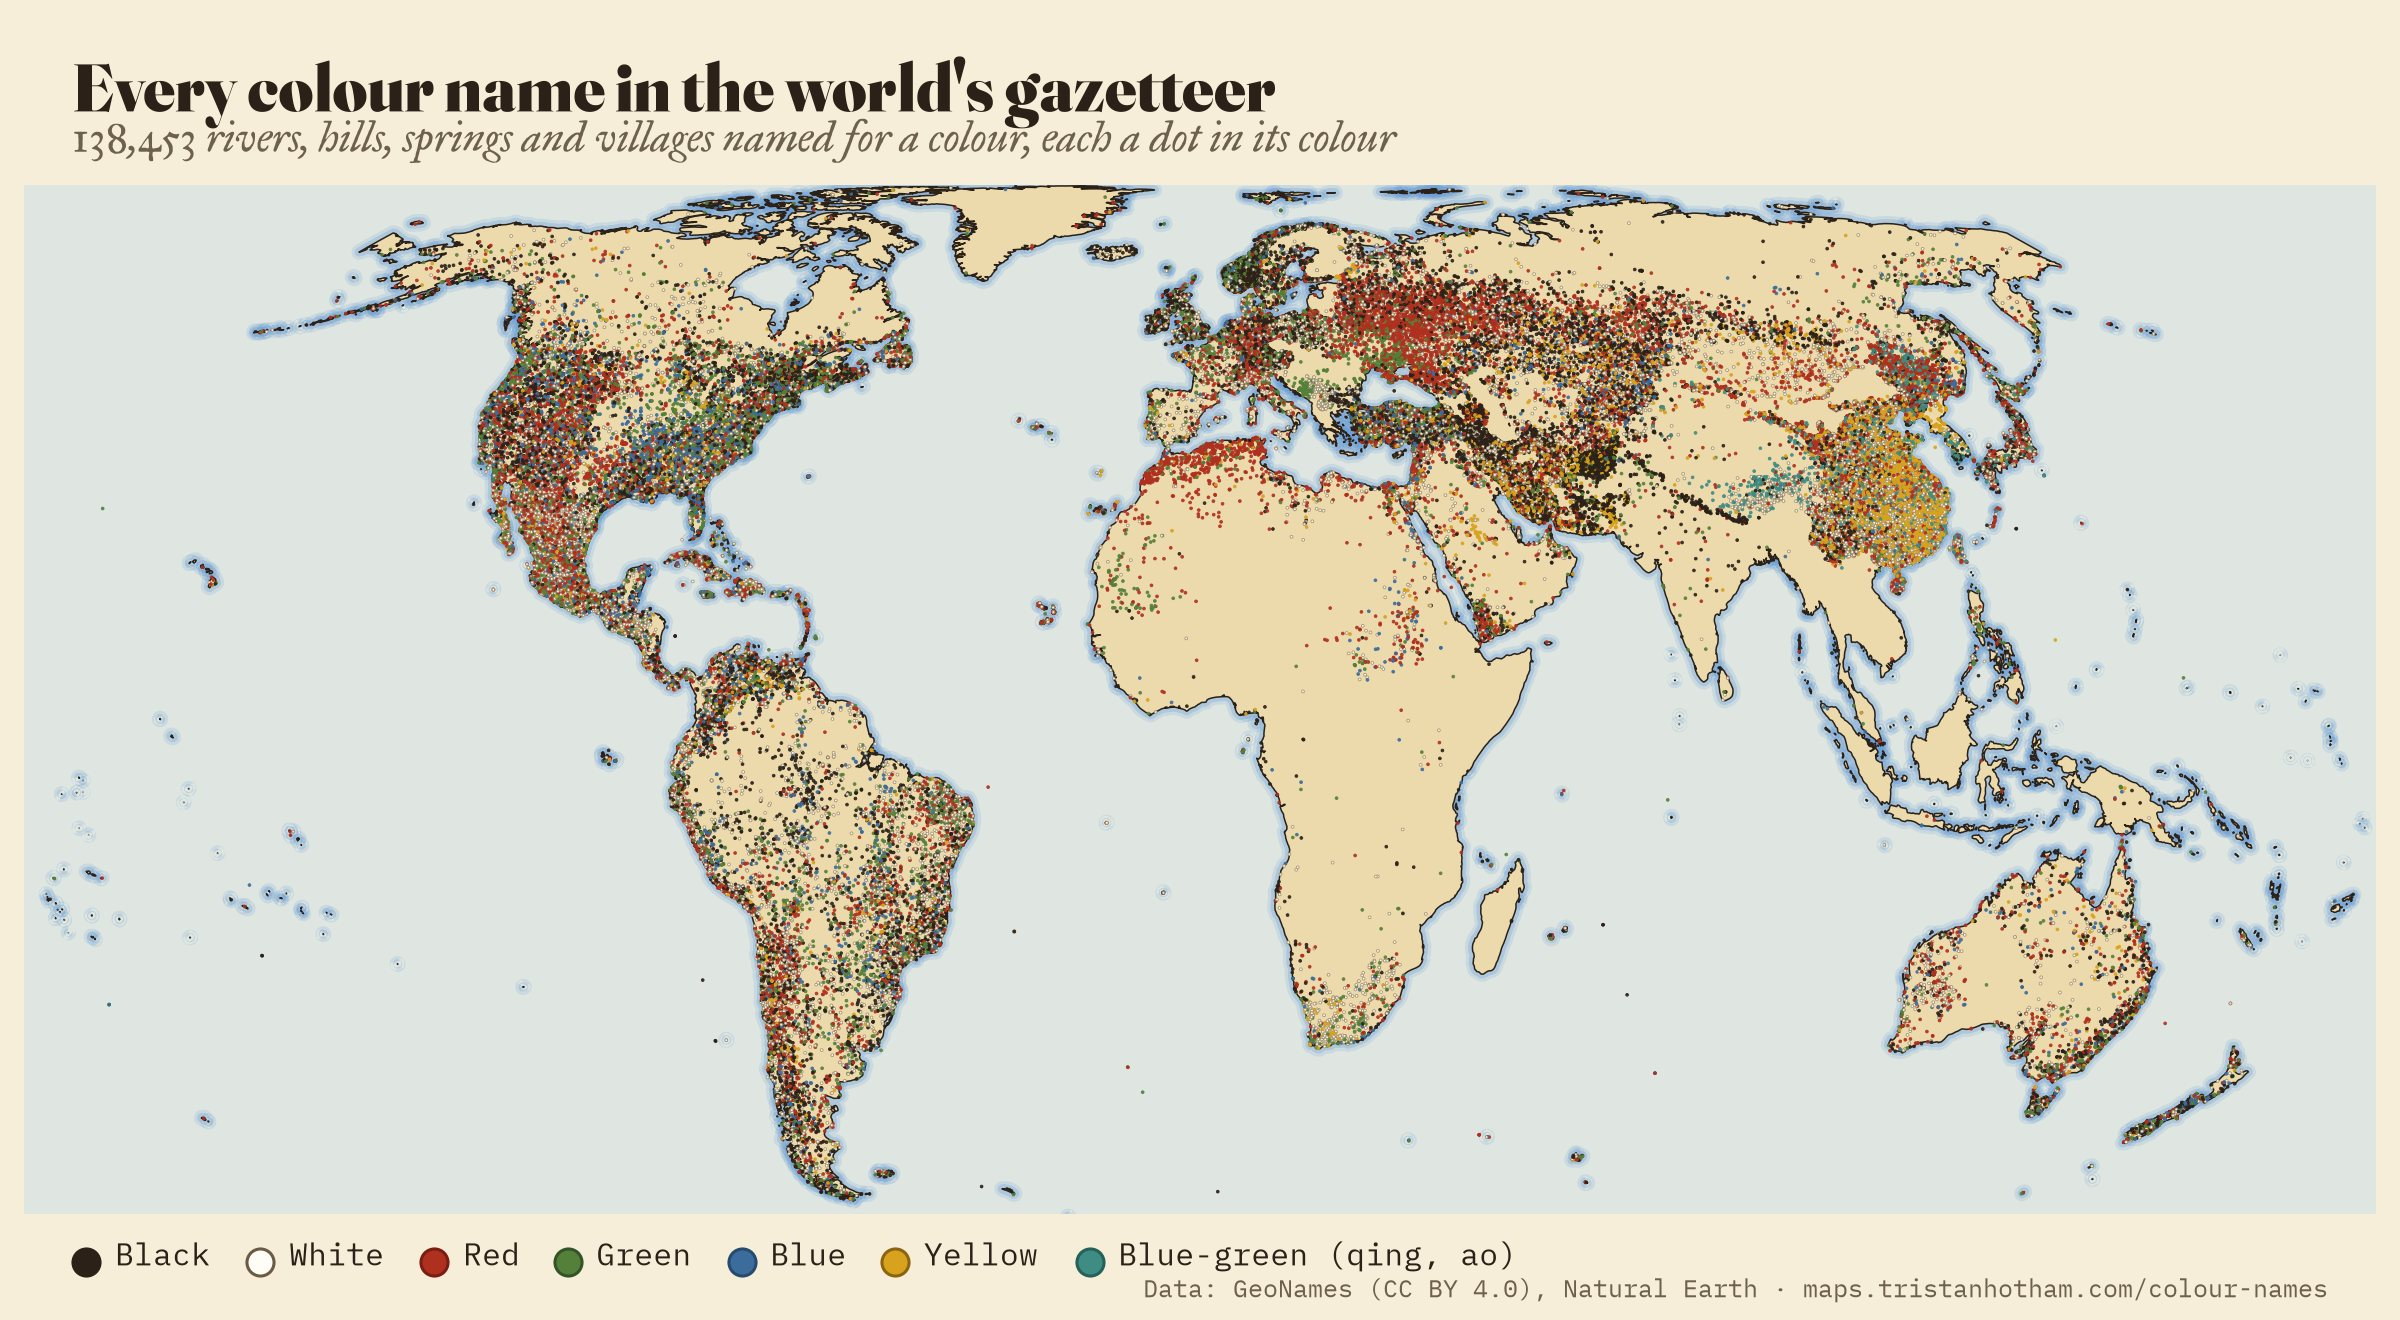
\includegraphics[width=\textwidth]{f_world.jpg}
\caption{Every colour name in the main set, a dot in its colour (Equal Earth projection).}\label{fig:world}\end{figure}

\subsection{Which colours}
White is the commonest colour (26.5\%), then black (23.2\%), red (20.6\%), yellow (10.7\%), green (10.5\%), blue-green (3.0\%) and blue (5.5\%). Yellow's place owes everything to China: without Chinese and Japanese names the order is black 27.3\%, white 25.7\%, red 21.3\%, green 13.1\%, blue 6.9\% and yellow 5.6\%. Black, white and red together make up more than half of the colour names of every language with at least 300 names, matching the first stages of \citet{berlinkay}; blue is never among the three commonest of the six colours in any such language (Figure~\ref{fig:mix}).

\begin{figure}[tbp]\centering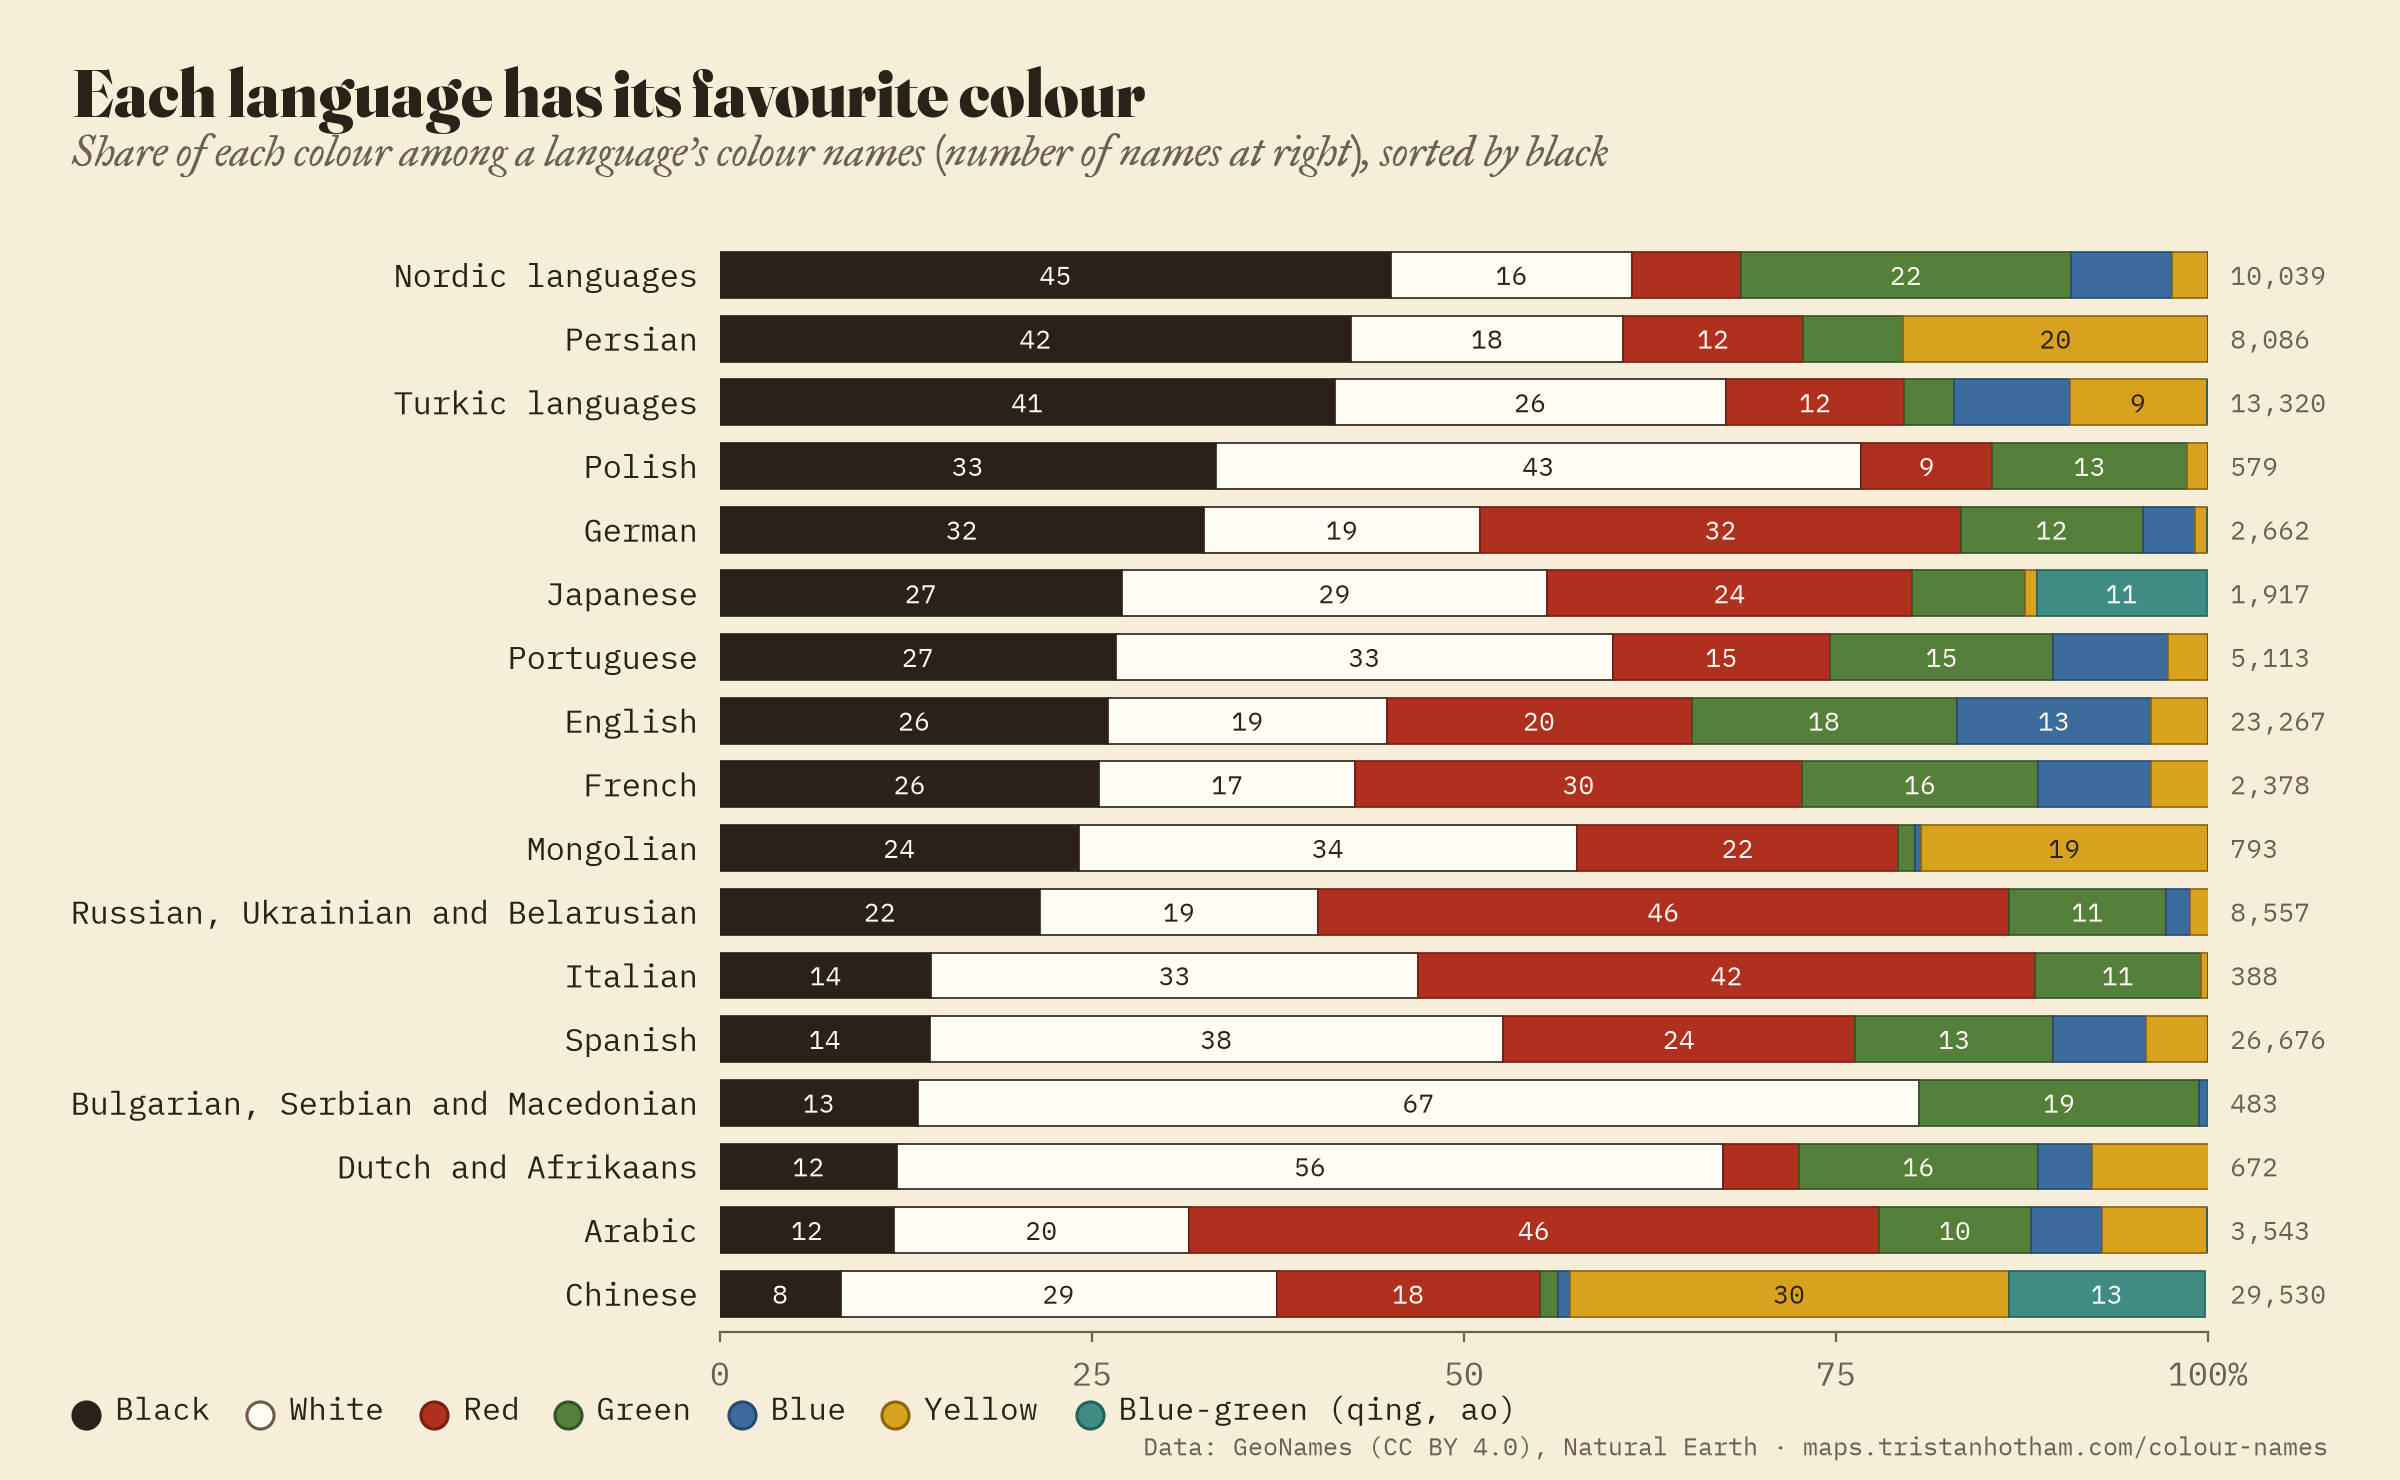
\includegraphics[width=\textwidth]{f_mix.png}
\caption{Share of each colour among the colour names of each language with at least 300 names.}\label{fig:mix}\end{figure}

\subsection{Which places}
With languages weighted equally (Figure~\ref{fig:kinds}, Table~\ref{tab:kinds}), rivers and streams are the blackest kind of place (37.2\% black against 29.1\% white), and rivers are blacker than their language's average in 14 of 17 languages. Springs and wells are the whitest (42.7\%). Red reaches its highest share on rocks, cliffs and islands. Mountains are white more often than black (28.4\% against 27.6\%, with red at 23.4\%), but they are whiter than their language's average in only 7 of 16 languages; they are whiter than average in Chinese, Japanese, Mongolian, Dutch and Afrikaans, Russian, the Nordic languages and French, but not in Spanish, German, English, Persian or the Turkic languages. The ratio of black to white names is 1.28 for rivers, 1.03 for lakes and 1.13 for seas and coasts, but 0.35 for springs and 0.84 for settlements.

\begin{figure}[tbp]\centering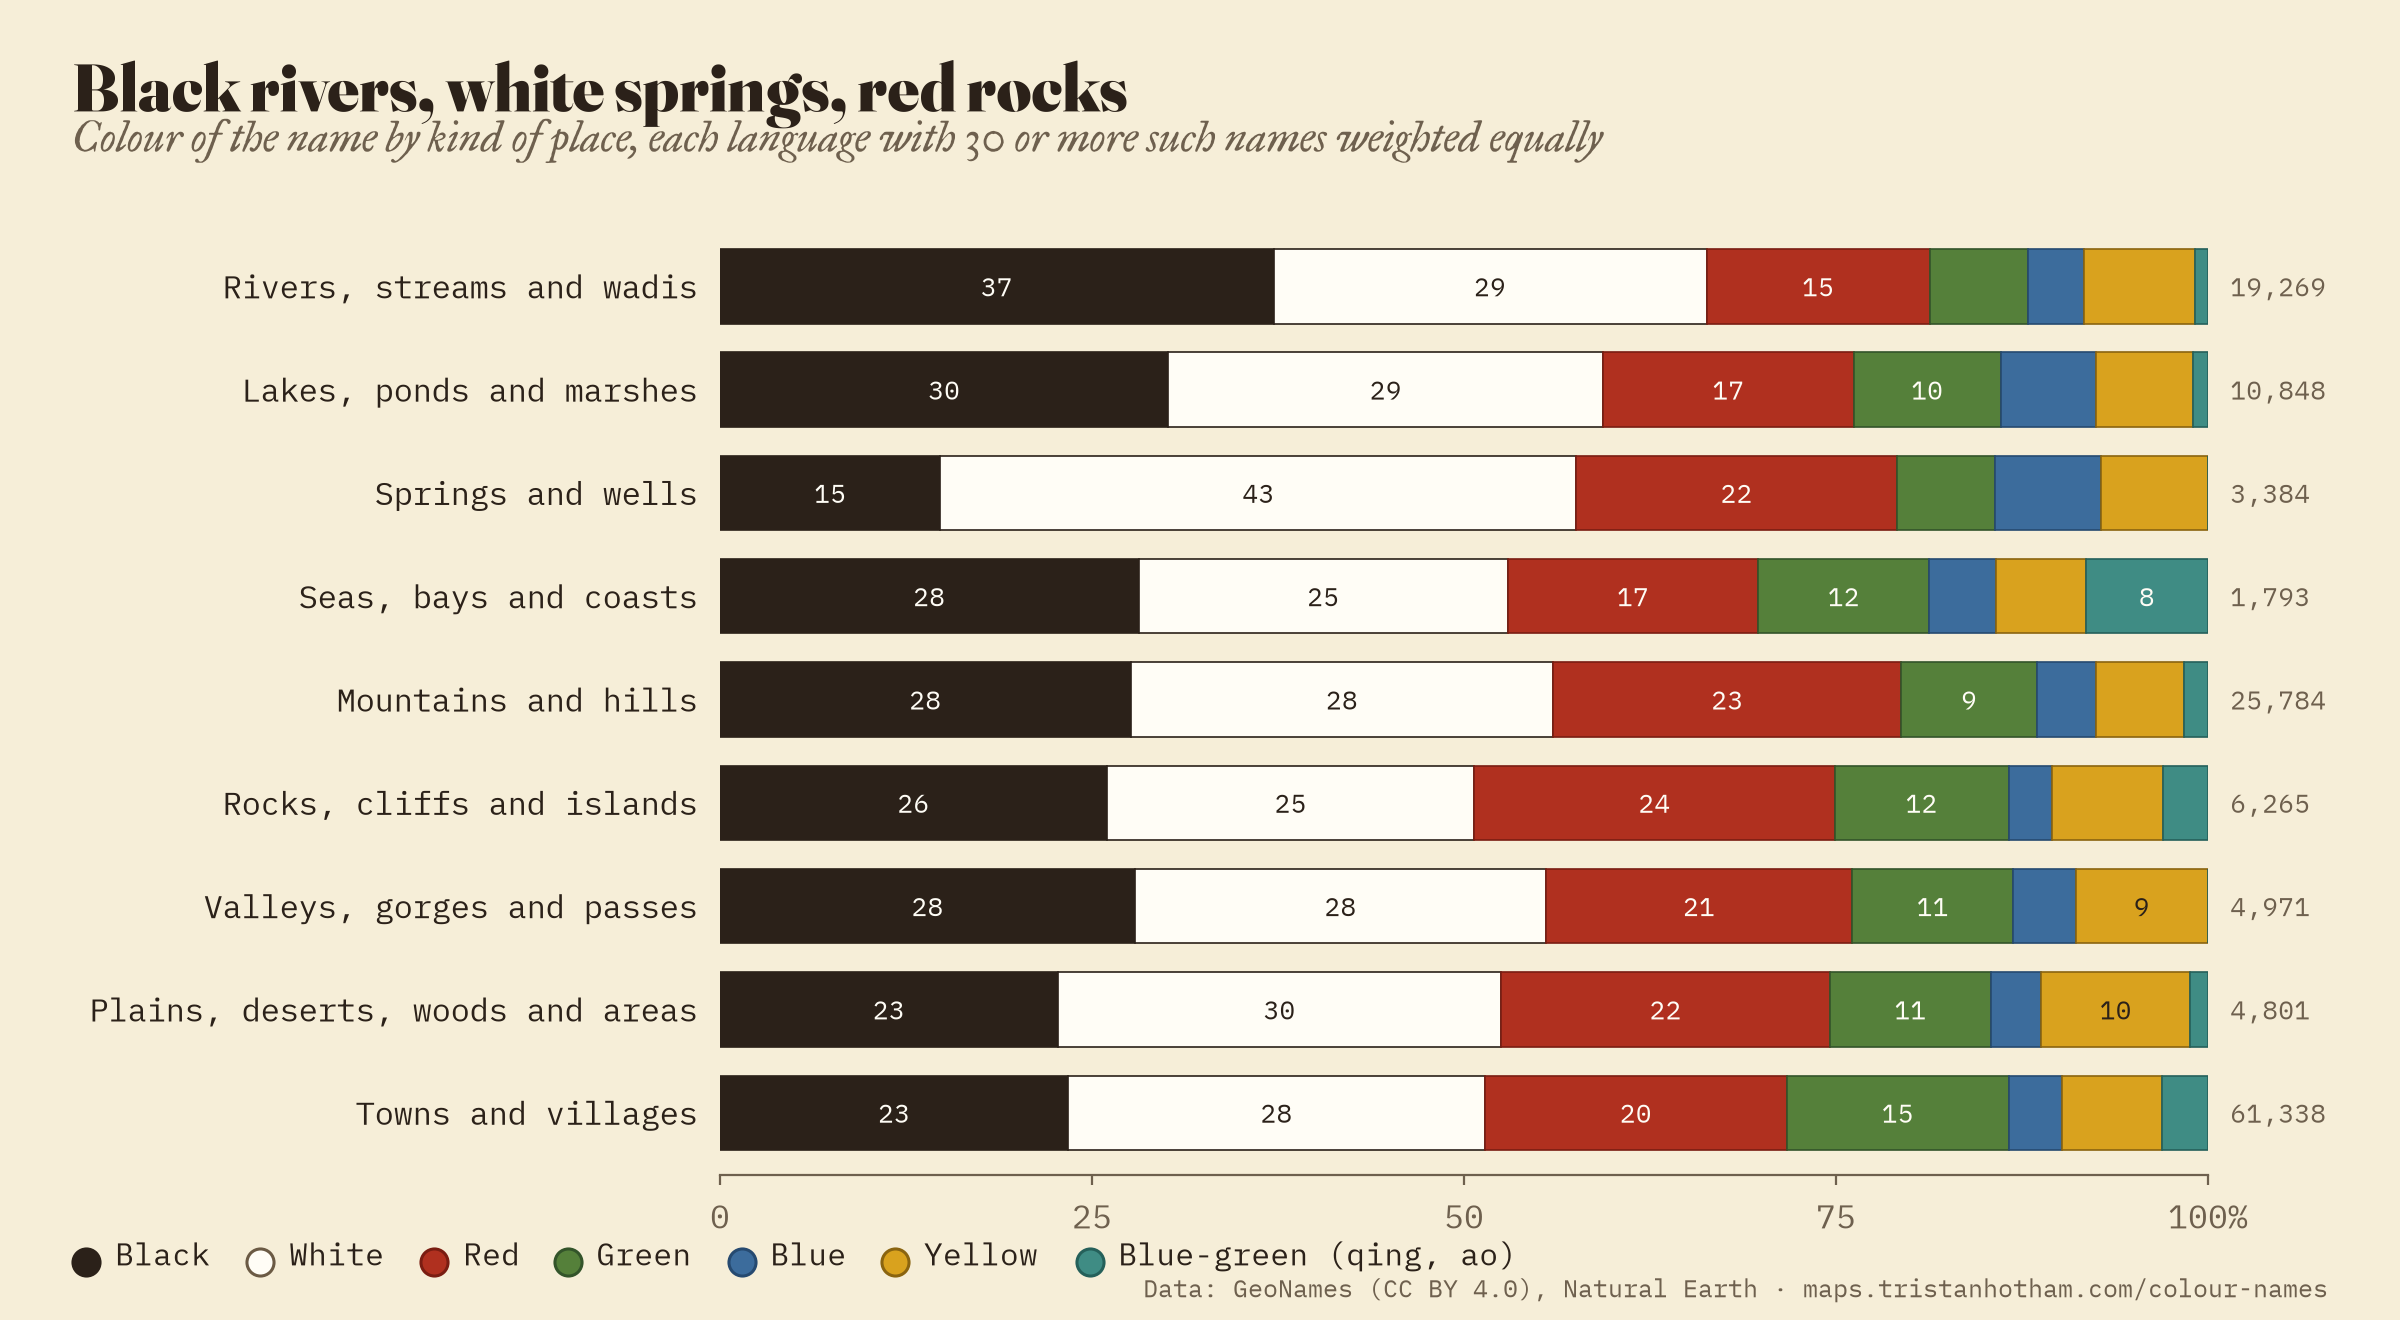
\includegraphics[width=\textwidth]{f_kinds.png}
\caption{Colour of the name by kind of place, languages with at least 30 names of that kind weighted equally.}\label{fig:kinds}\end{figure}

\begin{table}[tbp]\centering\footnotesize\caption{Colour by kind of place: names in the main set, and the share of each colour (\%) with languages weighted equally. BG: blue-green.}\label{tab:kinds}\begin{tabular}{lrrrrrrrr}\toprule Kind & Names & Black & White & Red & Green & Blue & Yellow & BG\\\midrule
Rivers, streams and wadis & 19,269 & 37.2 & 29.1 & 15.0 & 6.6 & 3.8 & 7.4 & 0.9\\
Lakes, ponds and marshes & 10,848 & 30.1 & 29.2 & 16.8 & 9.9 & 6.4 & 6.5 & 1.0\\
Springs and wells & 3,384 & 14.8 & 42.7 & 21.5 & 6.6 & 7.1 & 7.2 & 0.0\\
Seas, bays and coasts & 1,793 & 28.1 & 24.8 & 16.8 & 11.5 & 4.5 & 6.0 & 8.2\\
Mountains and hills & 25,784 & 27.6 & 28.4 & 23.4 & 9.1 & 4.0 & 5.9 & 1.6\\
Rocks, cliffs and islands & 6,265 & 26.0 & 24.7 & 24.2 & 11.7 & 2.9 & 7.5 & 3.0\\
Valleys, gorges and passes & 4,971 & 27.9 & 27.6 & 20.6 & 10.8 & 4.2 & 8.9 & 0.0\\
Plains, deserts, woods and areas & 4,801 & 22.7 & 29.8 & 22.1 & 10.8 & 3.4 & 10.0 & 1.2\\
Towns and villages & 61,338 & 23.4 & 28.0 & 20.3 & 14.9 & 3.6 & 6.7 & 3.1\\
\bottomrule\end{tabular}\end{table}

\subsection{Languages and their favourite colours}
Table~\ref{tab:langs} sets out the colour mix of each language. In the Nordic languages 45.1\% of colour names are svart, black, mostly lakes, tarns and fells; in Persian and Dari 42.4\% are siāh, and Kūh-e Sīāh, Black Mountain, occurs 284 times. In the Turkic languages kara and ak make up 67.7\% of colour names, and Karasu, black water, occurs 239 times. Mongolian favours white (33.5\%, \textit{tsagaan}), then black (24.1\%, \textit{khar}, mostly in Buryatia) and red (21.6\%, \textit{ulaan}). Arabic (46.4\%) and the East Slavic languages (46.4\%) are the reddest: aḥmar and ḥamrā’ for desert rock and sand, krasnyy for villages. Spanish is the whitest of the large languages (38.5\% white), and the commonest colour name in the world is the Spanish Cerro Colorado (1,084 names), followed by Cerro Blanco (748) and Cerro Negro (531). Unlike most languages, Spanish and Portuguese rivers are whiter than black (36.4\% against 21.9\%; 428 Río Blanco against 309 Río Negro). In Chinese, bai (white, {\cjk 白}) and huang (yellow, {\cjk 黄}) make up 58.8\% of colour names (Figure~\ref{fig:families}).

\begin{table}[tbp]\centering\footnotesize\caption{Colour names by language: names in the main set, share of each colour (\%) and the share of review-sample names judged correct (\%).}\label{tab:langs}\begin{tabular}{lrrrrrrrrr}\toprule Language & Names & Black & White & Red & Green & Blue & Yellow & BG & Correct\\\midrule
Chinese & 29,530 & 8 & 29 & 18 & 1 & 1 & 30 & 13 & 97\\
Spanish & 26,676 & 14 & 38 & 24 & 13 & 6 & 4 & 0 & 99\\
English & 23,267 & 26 & 19 & 20 & 18 & 13 & 4 & 0 & 97\\
Turkic languages & 13,320 & 41 & 26 & 12 & 3 & 8 & 9 & 0 & 99\\
Nordic languages & 10,039 & 45 & 16 & 7 & 22 & 7 & 2 & 0 & 99\\
Russian, Ukrainian and Belarusian & 8,557 & 22 & 19 & 46 & 11 & 2 & 1 & 0 & 100\\
Persian & 8,086 & 42 & 18 & 12 & 7 & 0 & 20 & 0 & 100\\
Portuguese & 5,113 & 27 & 33 & 15 & 15 & 8 & 3 & 0 & 99\\
Arabic & 3,543 & 12 & 20 & 46 & 10 & 5 & 7 & 0 & 99\\
German & 2,662 & 32 & 19 & 32 & 12 & 4 & 1 & 0 & 100\\
French & 2,378 & 26 & 17 & 30 & 16 & 8 & 4 & 0 & 99\\
Japanese & 1,917 & 27 & 29 & 24 & 8 & 0 & 1 & 11 & 99\\
Mongolian & 793 & 24 & 34 & 22 & 1 & 0 & 19 & 0 & nan\\
Dutch and Afrikaans & 672 & 12 & 56 & 5 & 16 & 4 & 8 & 0 & 100\\
Polish & 579 & 33 & 43 & 9 & 13 & 0 & 1 & 0 & 100\\
Bulgarian, Serbian and Macedonian & 483 & 13 & 67 & 0 & 19 & 1 & 0 & 0 & 100\\
Italian & 388 & 14 & 33 & 42 & 11 & 0 & 0 & 0 & 98\\
Hindi, Urdu and Nepali & 238 & 83 & 2 & 8 & 4 & 1 & 1 & 0 & nan\\
Korean & 184 & 15 & 15 & 0 & 0 & 0 & 38 & 32 & nan\\
Romanian & 28 & 0 & 0 & 0 & 100 & 0 & 0 & 0 & 100\\
\bottomrule\end{tabular}\end{table}

\begin{figure}[tbp]\centering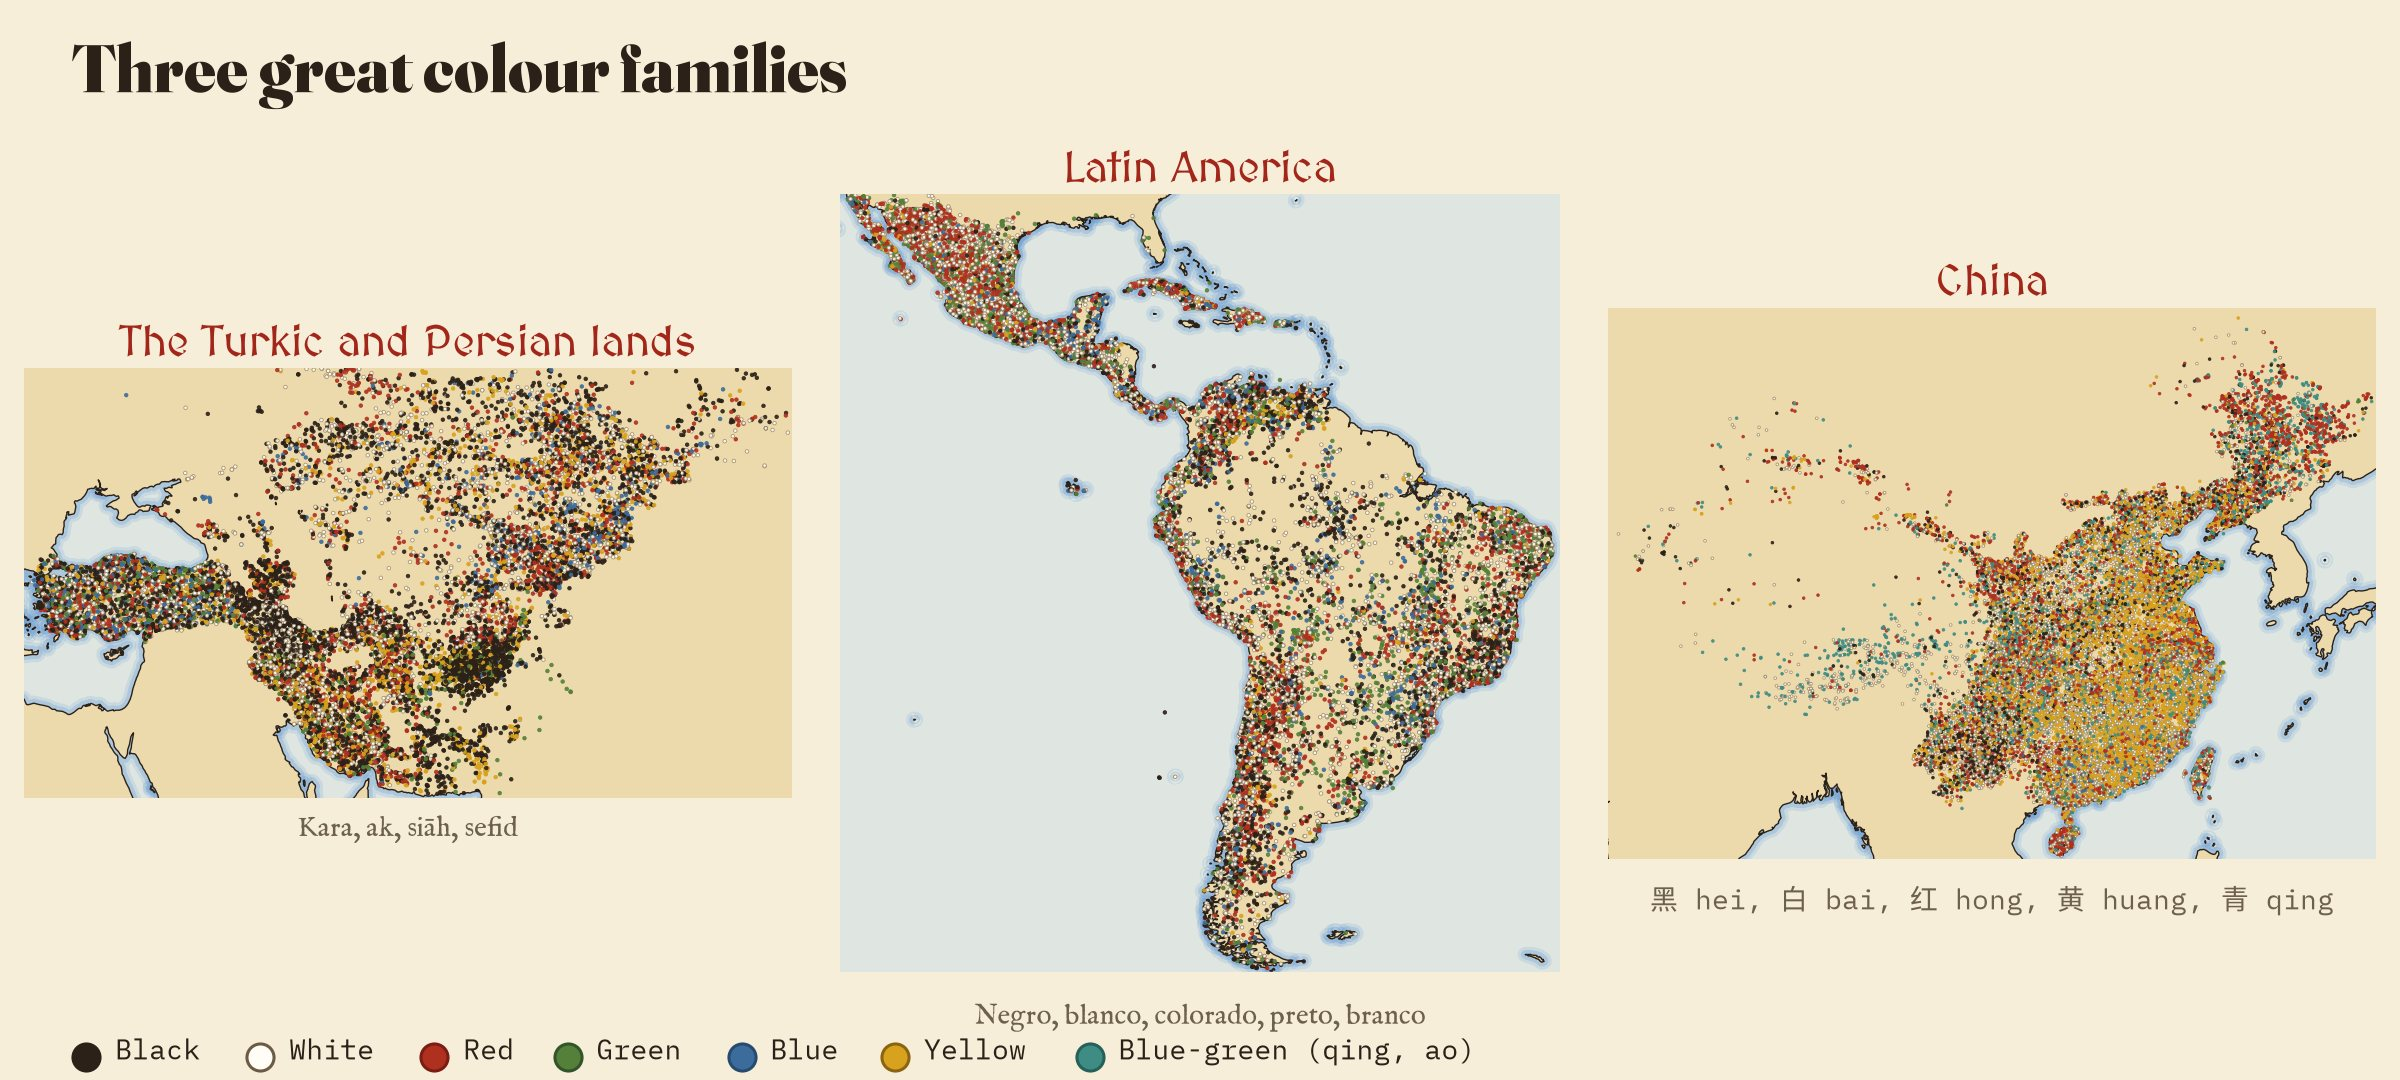
\includegraphics[width=\textwidth]{f_families.jpg}
\caption{Three colour families: the Turkic and Persian lands, Latin America and China (plate carrée at each panel's middle latitude).}\label{fig:families}\end{figure}

\subsection{Countries}
In the 102 countries with at least 30 names, the commonest colour is white in 35, black in 35, red in 21, green in 8, yellow in 2 and blue-green in 1 (South Korea); blue leads in none (Figure~\ref{fig:countries}). Black leads in the English-speaking countries, the Nordic countries, Turkey, Central Asia, Iran and Afghanistan; white in most of Latin America, Mongolia, Serbia, North Macedonia, Poland and South Africa; red in Russia, Belarus and much of the Arab world; yellow in China. By the ratio of black to white names (Figure~\ref{fig:bw}), 41 countries have more black than white names and 57 more white than black. With \textit{kvit} from the second pass, Norway's ratio is 2.8 to one. The most extreme ratios now come from the narrow Hindi and Urdu rule: India (32.6) and Pakistan (30.6) look very black because nearly all the names it accepts are \textit{kala}.

\begin{figure}[tbp]\centering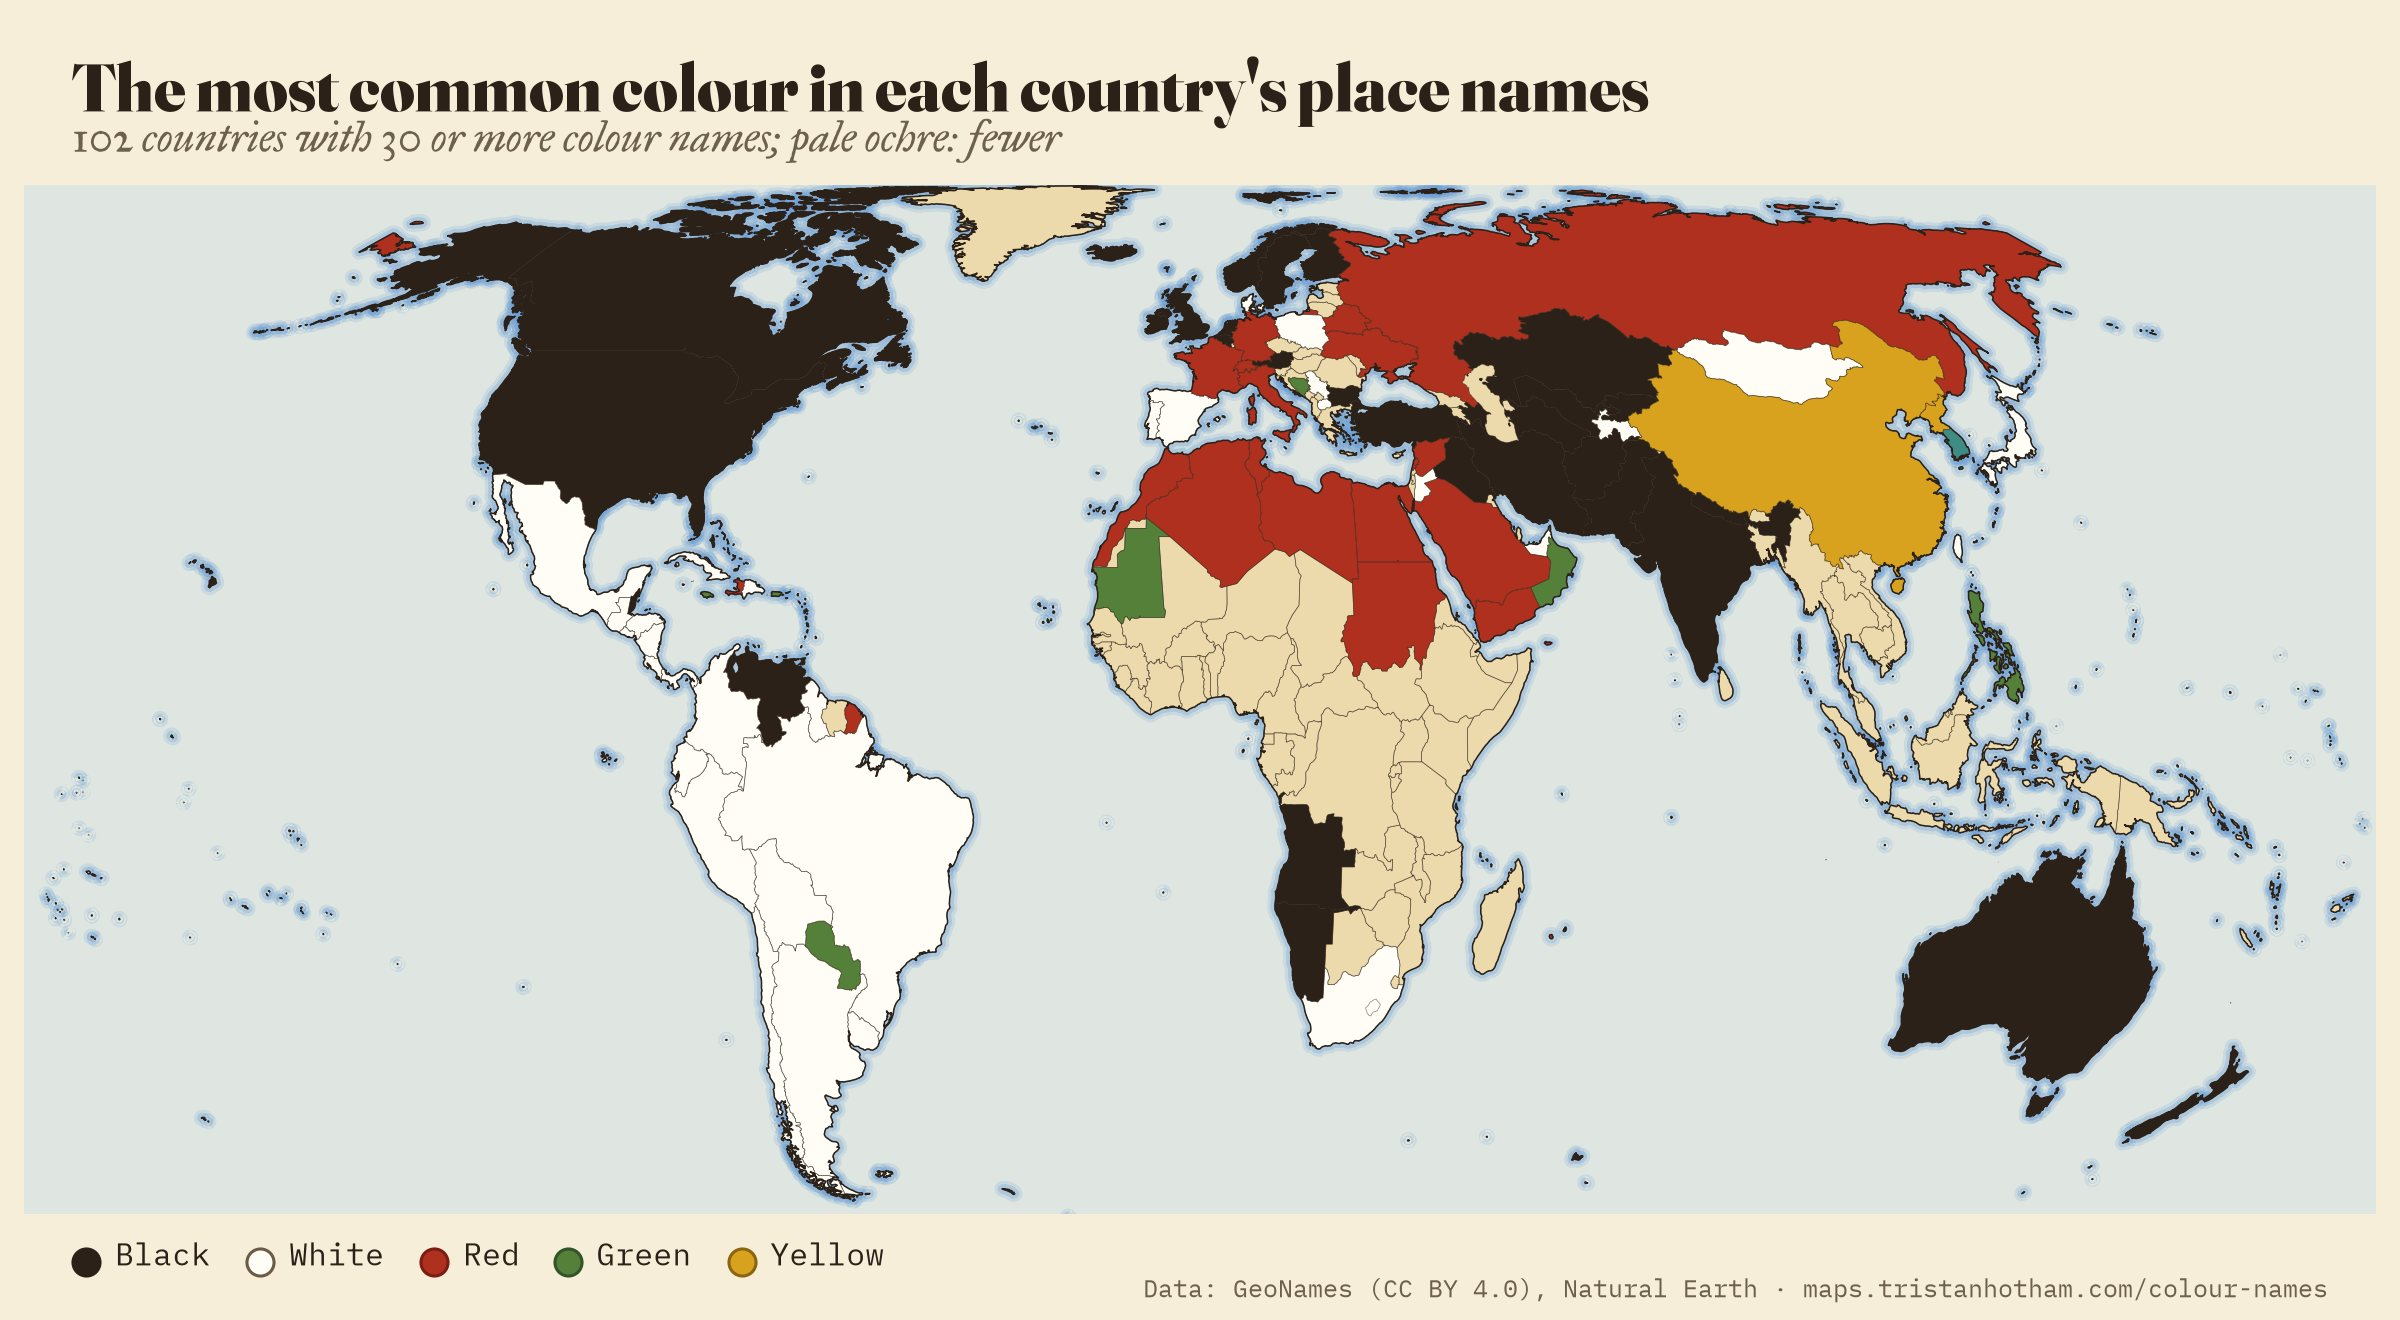
\includegraphics[width=\textwidth]{f_countries.jpg}
\caption{The commonest colour among each country's colour names, countries with at least 30 names.}\label{fig:countries}\end{figure}
\begin{figure}[tbp]\centering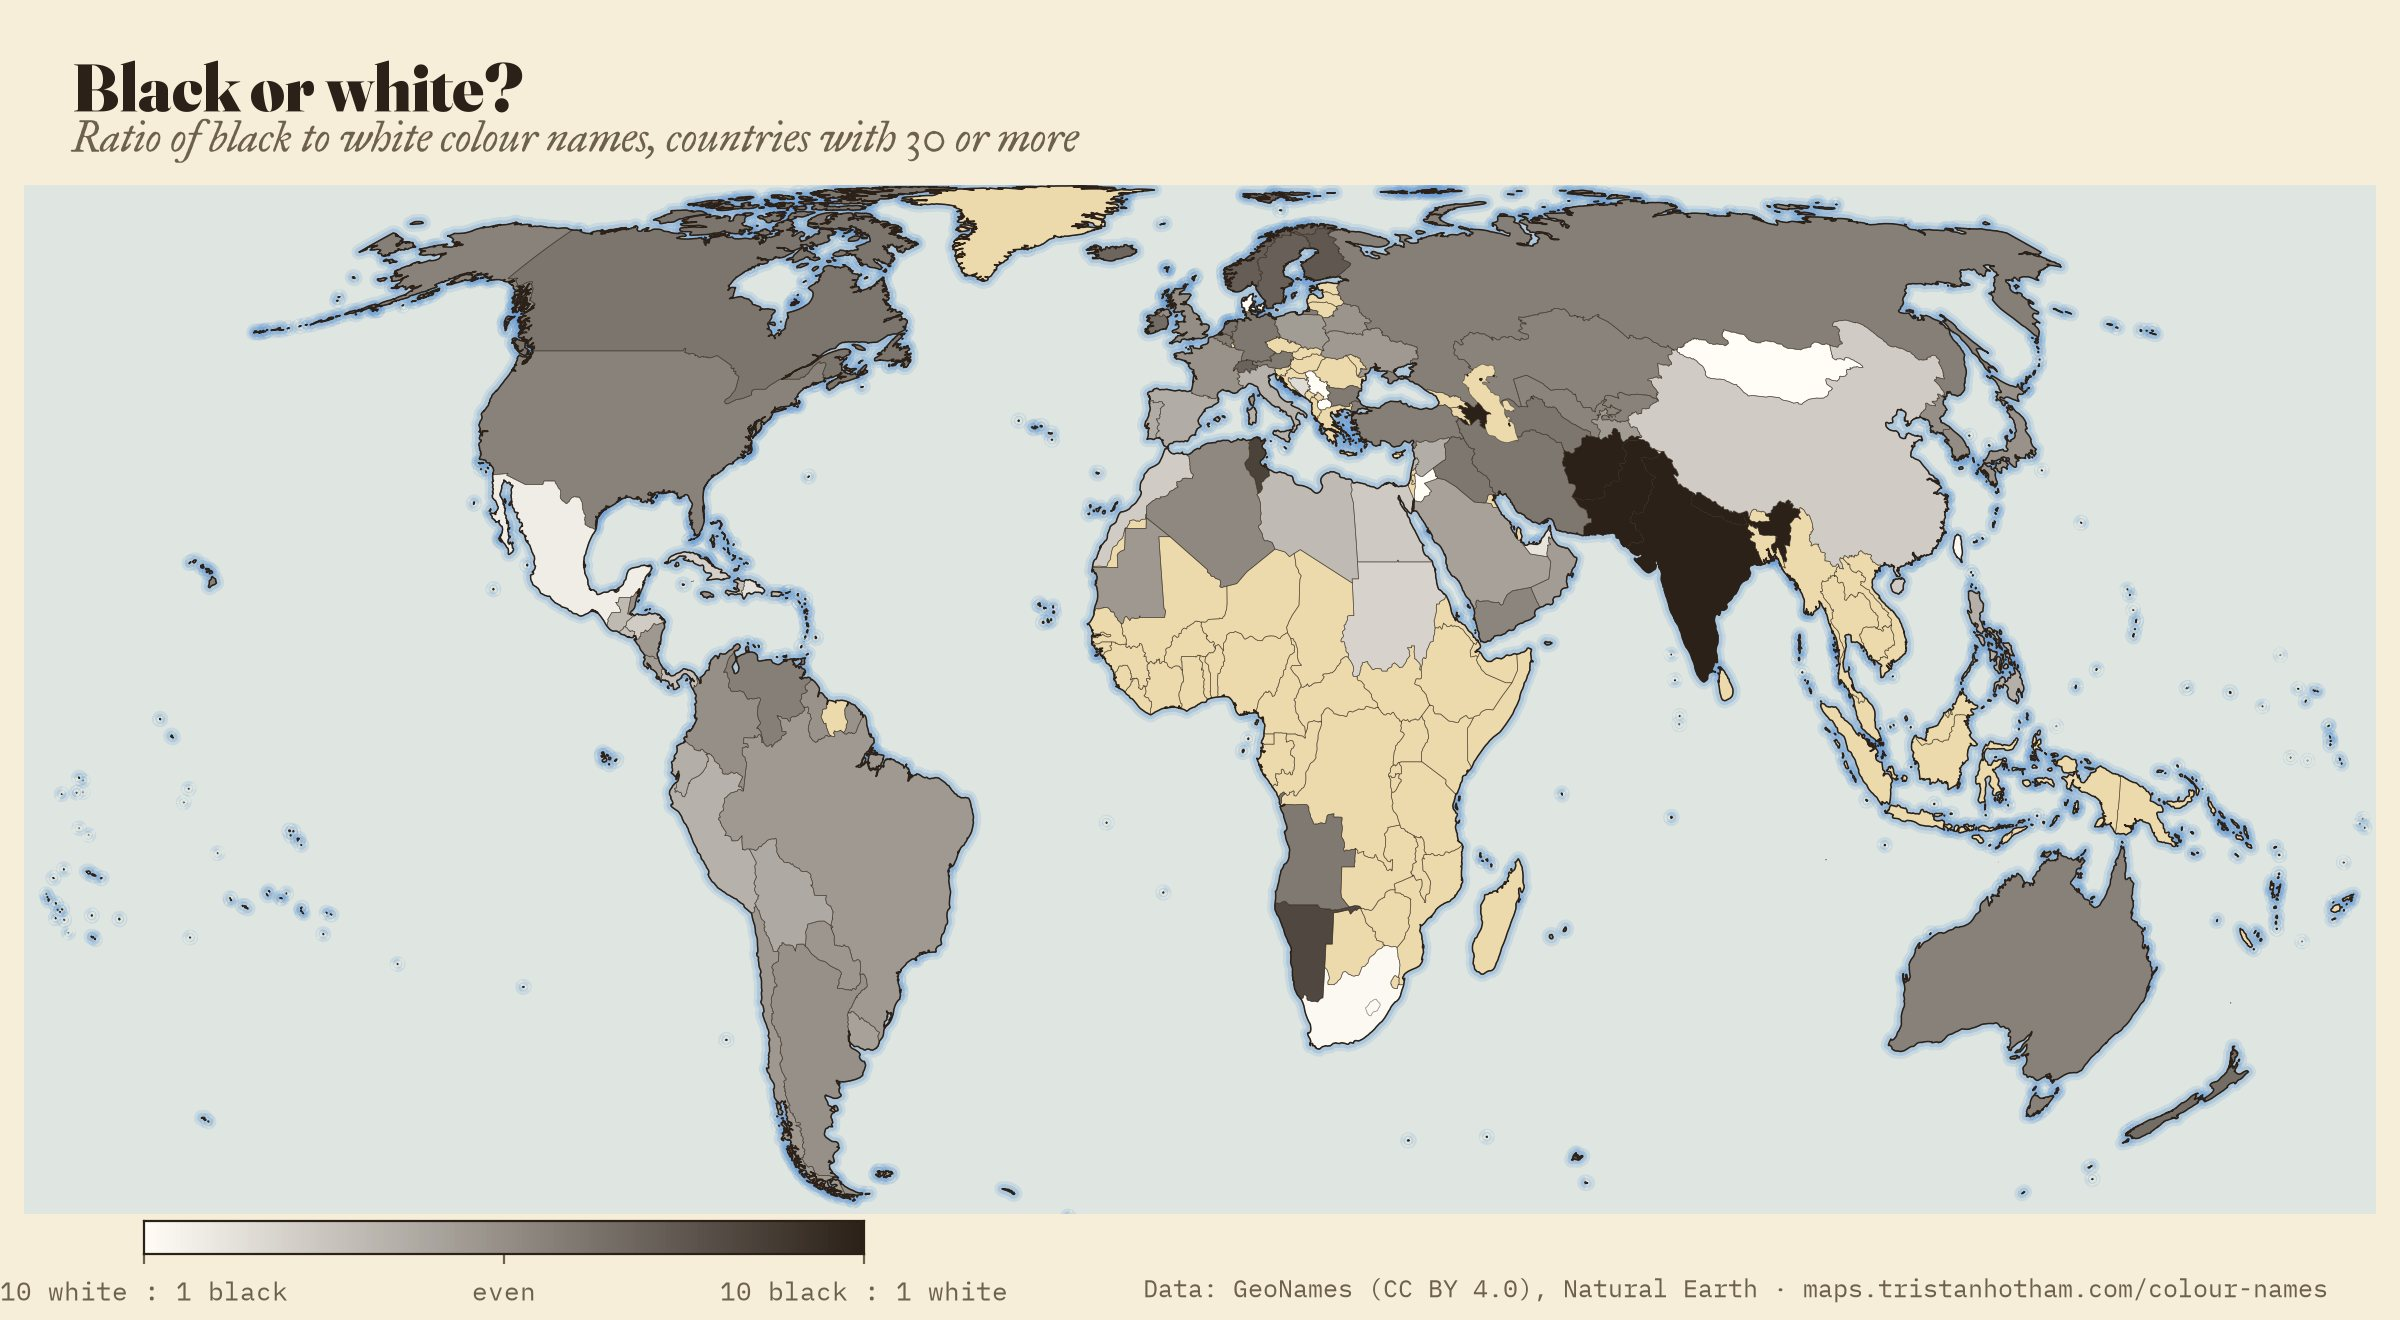
\includegraphics[width=\textwidth]{f_bw.jpg}
\caption{Ratio of black to white colour names, countries with at least 30 names (log scale).}\label{fig:bw}\end{figure}

\subsection{Hotspots}
On a two-degree grid the densest cell of black names is in central Norway (350 names), of white and red names in central Mexico (342 and 219), of green and blue names in western Norway, and of yellow names in southern China (288). These follow the gazetteer's density as much as naming habits.

\subsection{Red: revolution and earth}
Of 3,974 red names in Russian, Ukrainian and Belarusian, 871 (21.9\%) are revolutionary; of 5,241 Chinese red names, 1,561 (29.8\%). Without them, red would fall from 46.4\% to 40.4\% of East Slavic colour names. Some of the remaining East Slavic red is not colour at all: \textit{krasnyy} long meant beautiful, so a Krasnaya Polyana may be a fair glade. Of 3,735 names of earth, soil, sand and clay, 763 (20.4\%) are red, close to the share of red among all names (20.6\%); 1,247 are white (Tierra Blanca alone 406 times) and 1,200 yellow (Figure~\ref{fig:red}).

\begin{figure}[tbp]\centering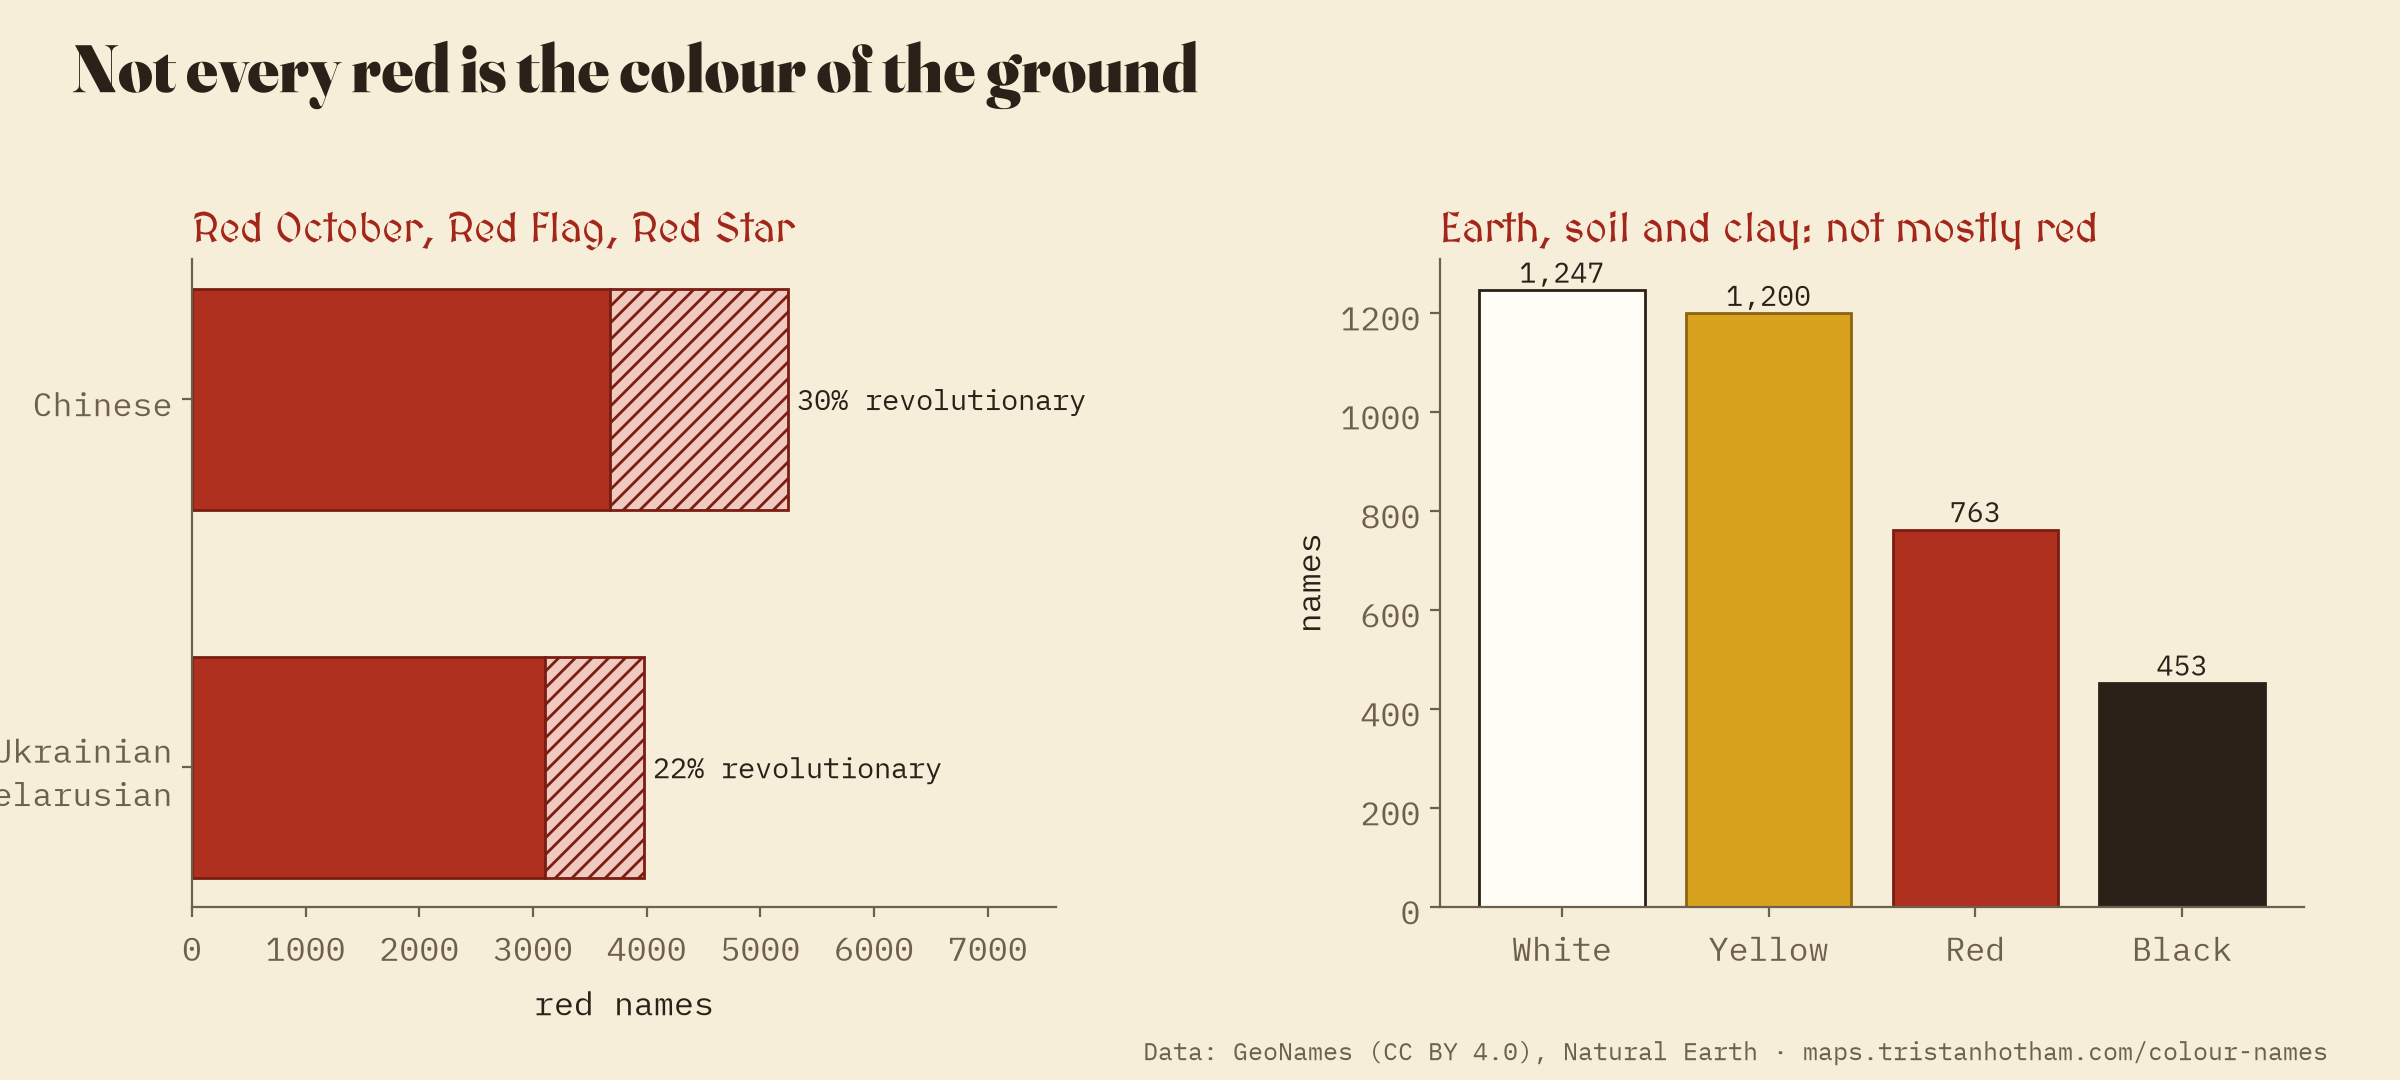
\includegraphics[width=\textwidth]{f_red.png}
\caption{Left: revolutionary red among East Slavic and Chinese red names. Right: colours of names of earth, soil, sand and clay.}\label{fig:red}\end{figure}

\subsection{Precision}
After tuning, 4,327 of 4,370 sampled names were judged correct (99\%; 0.98 when each language and colour cell is weighted by its number of names). The lowest cell with at least 20 names sampled reaches 0.92. English (0.97) and Chinese (0.97) are the weakest languages, for family names and names written in sound (Figure~\ref{fig:precision}).

\begin{figure}[tbp]\centering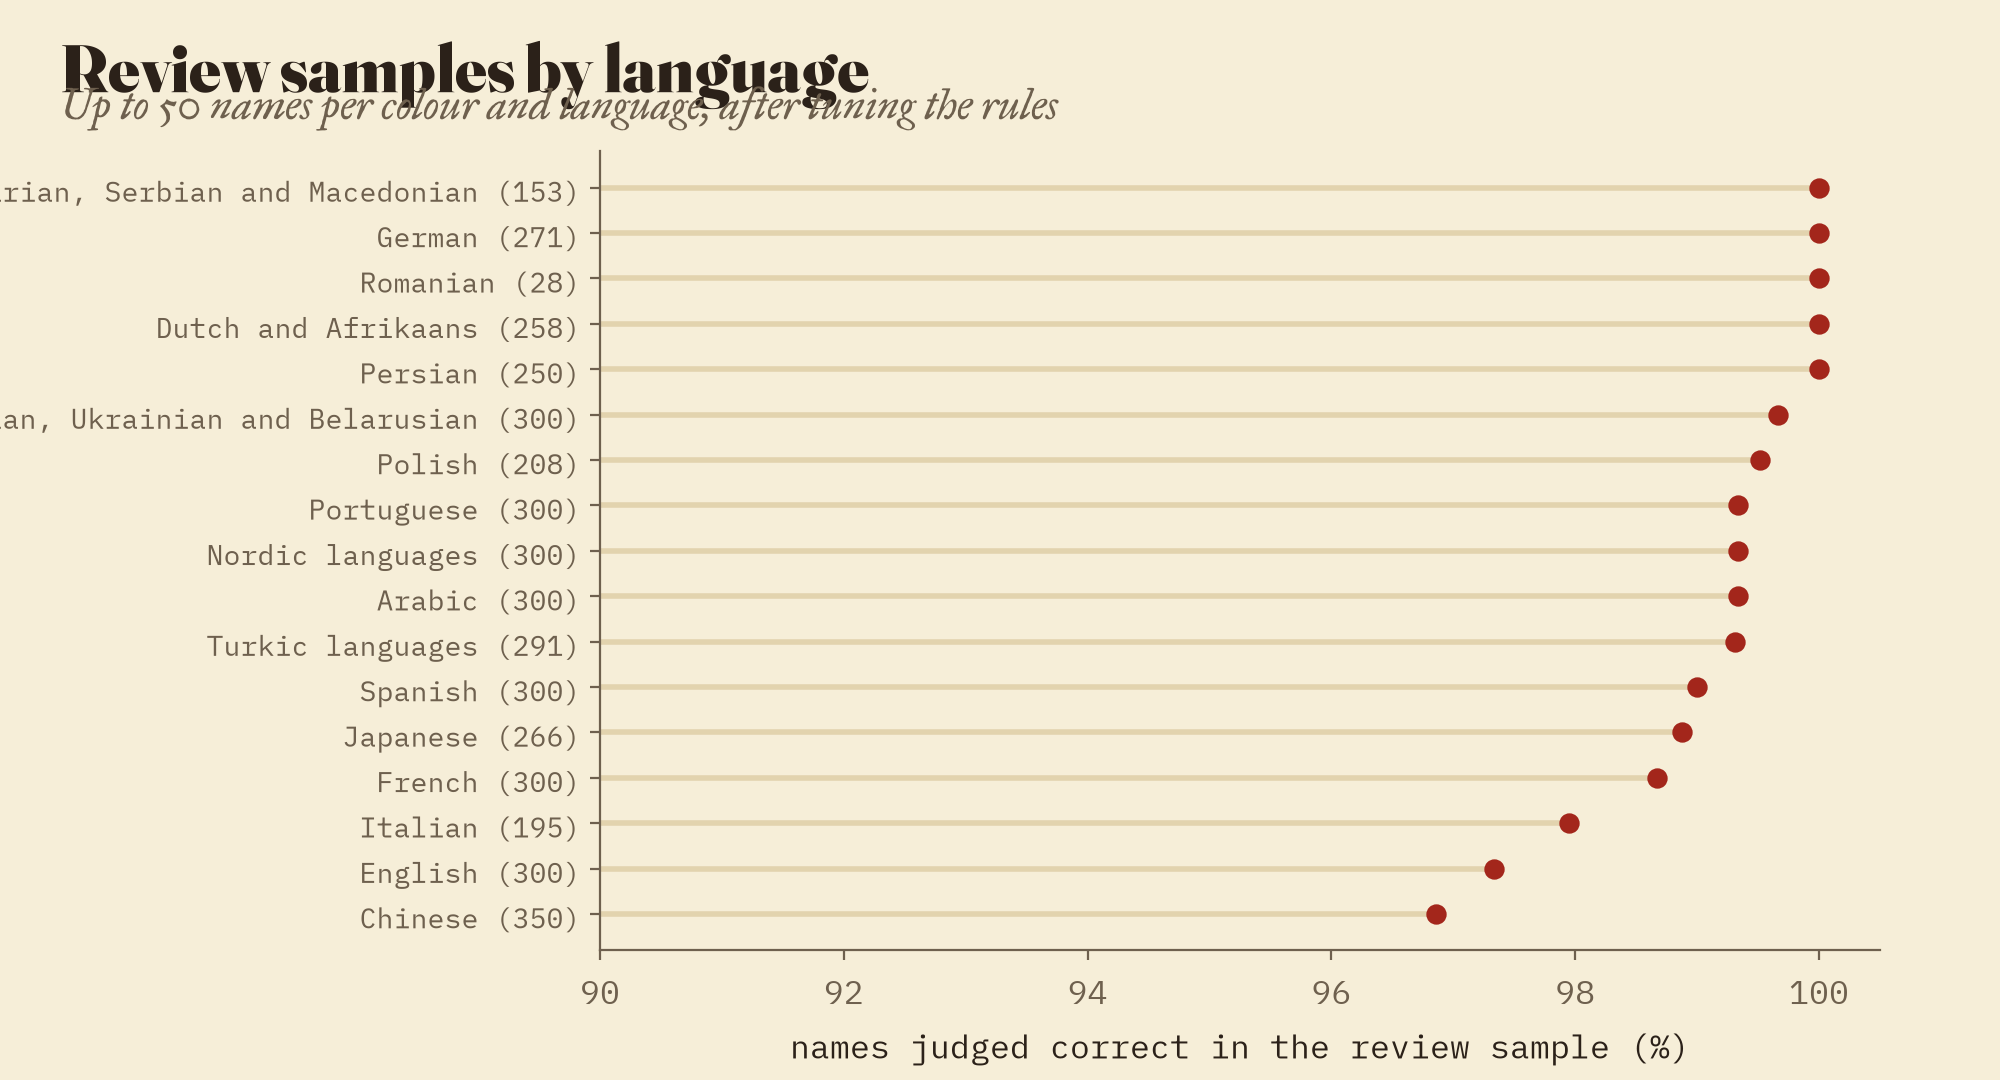
\includegraphics[width=0.85\textwidth]{f_precision.png}
\caption{Names judged correct in the review samples, by language (names sampled in brackets).}\label{fig:precision}\end{figure}

\section{Limitations}
First, recall is limited by the searches that produced the candidates and by the strictness of the rules. The second pass filled the largest gaps of the first (English and Turkic compounds, Norwegian \textit{kvit}, Mongolian), but Korean, Hindi and Urdu are covered only where the meaning is clear, which favours some colours (black in South Asia); Afrikaans \textit{rooi} and \textit{swart}, Persian \textit{kabud}, and whole languages (Hungarian, Finnish, Greek, Malay and Indonesian, Pashto and the languages of Africa) are missing. The second pass was reviewed with only 50 names per rule. Second, GeoNames is uneven: counts follow the density of national gazetteers and include duplicates of the same feature. Third, precision is measured on samples that also guided the rules, so it is optimistic, and some judgements are uncertain: whether a Spanish \textit{Loma Los Negros} names the colour or people, or a Chinese {\cjk 黄} village a family. Fourth, a colour word does not tell us why the place was so named: Black can be peat, shade, a forest, a fearful reputation or a direction (in the Turkic tradition black has been read as north and white as west, \citealp{wikiblacksea}). Fifth, the six colours and blue-green are this study's categories, not the languages' own.

\section{Conclusion}
The colours of the world's place names follow the oldest colour words: white, black and red make up most of them, blue is rare. Each kind of place has a leaning, black for rivers and dark water, white for springs, red for rock and bare ground, and each language has its favourite word, from svart and siāh to blanco and huang. A good part of the red, though, is not the colour of the land but of twentieth-century flags.

\section*{Data and code availability}
The interactive map is at \url{https://maps.tristanhotham.com/colour-names/}. Data and code are at \url{https://github.com/Tristan-Hotham/colour-names} and archived with this paper at https://doi.org/10.5281/zenodo.24043682. Derived data are released under CC BY 4.0 and code under the MIT licence. Place names are from GeoNames (CC BY 4.0); country outlines from Natural Earth (public domain); the map style uses OpenStreetMap data (ODbL).

\section*{AI statement}
I wrote the text, with drafting and editing assistance from Claude (Anthropic), which also helped prepare the analysis code. I reviewed and checked all text and results.

\begin{thebibliography}{9}
\bibitem[Berlin and Kay(1969)]{berlinkay} Berlin, B. and Kay, P. (1969) \textit{Basic Color Terms: Their Universality and Evolution}. Berkeley: University of California Press.
\bibitem[GeoNames(2026)]{geonames} GeoNames (2026) GeoNames geographical database, allCountries dump. CC BY 4.0. \url{https://www.geonames.org/}
\bibitem[Hotham(2026)]{inkmap} Hotham, T. (2026) The Inked World: a zoomable hand-inked style world map from open data. \url{https://maps.tristanhotham.com/ink-map/}
\bibitem[Natural Earth(2026)]{naturalearth} Natural Earth (2026) Admin 0 countries and land, 1:50m. Public domain. \url{https://www.naturalearthdata.com/}
\bibitem[\v{S}avri\v{c} et al.(2019)]{equalearth} \v{S}avri\v{c}, B., Patterson, T. and Jenny, B. (2019) The Equal Earth map projection. \textit{International Journal of Geographical Information Science} 33(3), 454 to 465.
\bibitem[Wikipedia(2026)]{wikiblacksea} Wikipedia contributors (2026) Black Sea: name. CC BY-SA 4.0. \url{https://en.wikipedia.org/wiki/Black_Sea}
\end{thebibliography}

\clearpage
\appendix
\section{The classifier's colour words}
{\footnotesize\setlength{\tabcolsep}{4pt}\begin{longtable}{p{2.6cm}p{6.6cm}p{5.4cm}}\caption{Colour words (dictionary forms; inflected and compound forms are also matched) and the countries where each rule applies.}\label{tab:rules}\\\toprule Language & Words & Where\\\midrule\endfirsthead\toprule Language & Words & Where\\\midrule\endhead
English & black: black; white: white; red: red; green: green; blue: blue; yellow: yellow & anywhere\\
Spanish & black: negro; white: blanco; red: rojo, colorado; green: verde; blue: azul; yellow: amarillo & anywhere outside the Portuguese and Italian areas; in the US, Canada and Australia only with a Spanish word beside it\\
Portuguese & black: preto, negro; white: branco; red: vermelho; green: verde; blue: azul; yellow: amarelo & Brazil, Portugal, Angola, Mozambique, Cape Verde and other Lusophone countries\\
French & black: noir; white: blanc; red: rouge; green: vert; blue: bleu; yellow: jaune & anywhere\\
Italian & black: nero; white: bianco; red: rosso; green: verde; yellow: giallo & Italy, San Marino, Switzerland\\
Romanian & green: verde & Romania, Moldova\\
German & black: schwarz; white: weiss; red: rot; green: grün; blue: blau; yellow: gelb & Germany, Austria, Switzerland, Liechtenstein, Luxembourg, Italy, Belgium, Namibia\\
Dutch and Afrikaans & black: zwart; white: wit; red: rood; green: groen; blue: blauw; yellow: geel & Netherlands, Belgium, Suriname, the Dutch Caribbean, South Africa, Namibia\\
Nordic languages & black: svart; white: hvit, vit; red: rød, röd; green: grønn, grön; blue: blå; yellow: gul & Norway, Sweden, Denmark, Finland, Iceland, the Faroes, Greenland\\
Polish & black: czarny; white: biały; red: czerwony; green: zielony; blue: niebieski; yellow: żółty & Poland\\
Russian, Ukrainian and Belarusian & black: chërnyy; white: belyy; red: krasnyy; green: zelënyy; blue: siniy; yellow: zhëltyy & the former Soviet Union and Mongolia\\
Bulgarian, Serbian and Macedonian & black: cheren; white: bel; green: zelen; blue: sin & Bulgaria, Serbia, North Macedonia, Bosnia, Montenegro, Kosovo\\
Turkic languages & black: kara, qara; white: ak, aq; red: kızıl, kyzyl; green: yeşil; blue: gök, kök; yellow: sarı, sary & Turkey, the Caucasus, Central Asia, Russia, Iran, Afghanistan, China, Mongolia and the Balkans\\
Arabic & black: aswad, sawdā’; white: abyaḍ, bayḍā’; red: aḥmar, ḥamrā’; green: akhḍar, khaḍrā’; blue: azraq, zarqā’; yellow: aṣfar, ṣafrā’ & the Arab world, Chad, Mali, Niger, Iran, Turkey (with an Arabic word beside it)\\
Persian & black: siāh; white: sefid; red: sorkh; green: sabz; yellow: zard & Iran, Afghanistan, Tajikistan, Pakistan\\
Chinese & black: {\cjk 黑} hei; white: {\cjk 白} bai; red: {\cjk 红} hong; green: {\cjk 绿} lü; blue: {\cjk 蓝} lan; yellow: {\cjk 黄} huang; grue: {\cjk 青} qing & China, Taiwan, Hong Kong, Macau (characters)\\
Japanese & black: {\cjk 黒} kuro; white: {\cjk 白} shiro; red: {\cjk 赤} aka; green: {\cjk 緑} midori; yellow: {\cjk 黄} ki; grue: {\cjk 青} ao & Japan (characters)\\
Mongolian & black: khar; white: tsagaan; red: ulaan; green: nogoon; blue: khökh; yellow: shar & Mongolia, Inner Mongolia, Buryatia, Kalmykia, Tuva\\
Hindi, Urdu and Nepali & black: kala; white: safed; red: lal; green: hara; blue: nila; yellow: pila & India, Pakistan, Nepal, Bangladesh (beside a landscape word)\\
Korean & black: {\cjk 黑} heuk; white: {\cjk 白} baek; red: {\cjk 紅} hong; green: {\cjk 綠} nok; yellow: {\cjk 黃} hwang; grue: {\cjk 靑} cheong & South and North Korea (hanja, or unambiguous hangul compounds)\\
\bottomrule\end{longtable}}

\section{The most repeated colour names}
{\footnotesize\begin{longtable}{llll}\caption{The 25 most repeated colour names in the main set.}\label{tab:top}\\\toprule Name & Colour & Language & Places\\\midrule\endfirsthead\toprule Name & Colour & Language & Places\\\midrule\endhead
Cerro Colorado & red & Spanish & 1,084\\
Cerro Blanco & white & Spanish & 748\\
Cerro Negro & black & Spanish & 527\\
Río Blanco & white & Spanish & 420\\
Red Hill & red & English & 415\\
Tierra Blanca & white & Spanish & 406\\
Agua Blanca & white & Spanish & 391\\
Casa Blanca & white & Spanish & 378\\
Black Creek & black & English & 375\\
Chërnaya & black & Russian, Ukrainian and Belarusian & 371\\
Palo Blanco & white & Spanish & 359\\
Black Mountain & black & English & 351\\
Cerro Verde & green & Spanish & 300\\
Arroyo Blanco & white & Spanish & 285\\
El Colorado & red & Spanish & 284\\
Kūh-e Sīāh & black & Persian & 284\\
Río Negro & black & Spanish & 278\\
Blue Lake & blue & English & 272\\
Black Lake & black & English & 263\\
Green Island & green & English & 252\\
Arroyo Colorado & red & Spanish & 247\\
Peña Blanca & white & Spanish & 242\\
Karasu & black & Turkic languages & 239\\
Loma Blanca & white & Spanish & 233\\
Ozero Beloye & white & Russian, Ukrainian and Belarusian & 233\\
\bottomrule\end{longtable}}
\end{document}
